\chapter*{Anexos}\label{chapter:annexes}

\begin{figure}[ht]
	\centering
	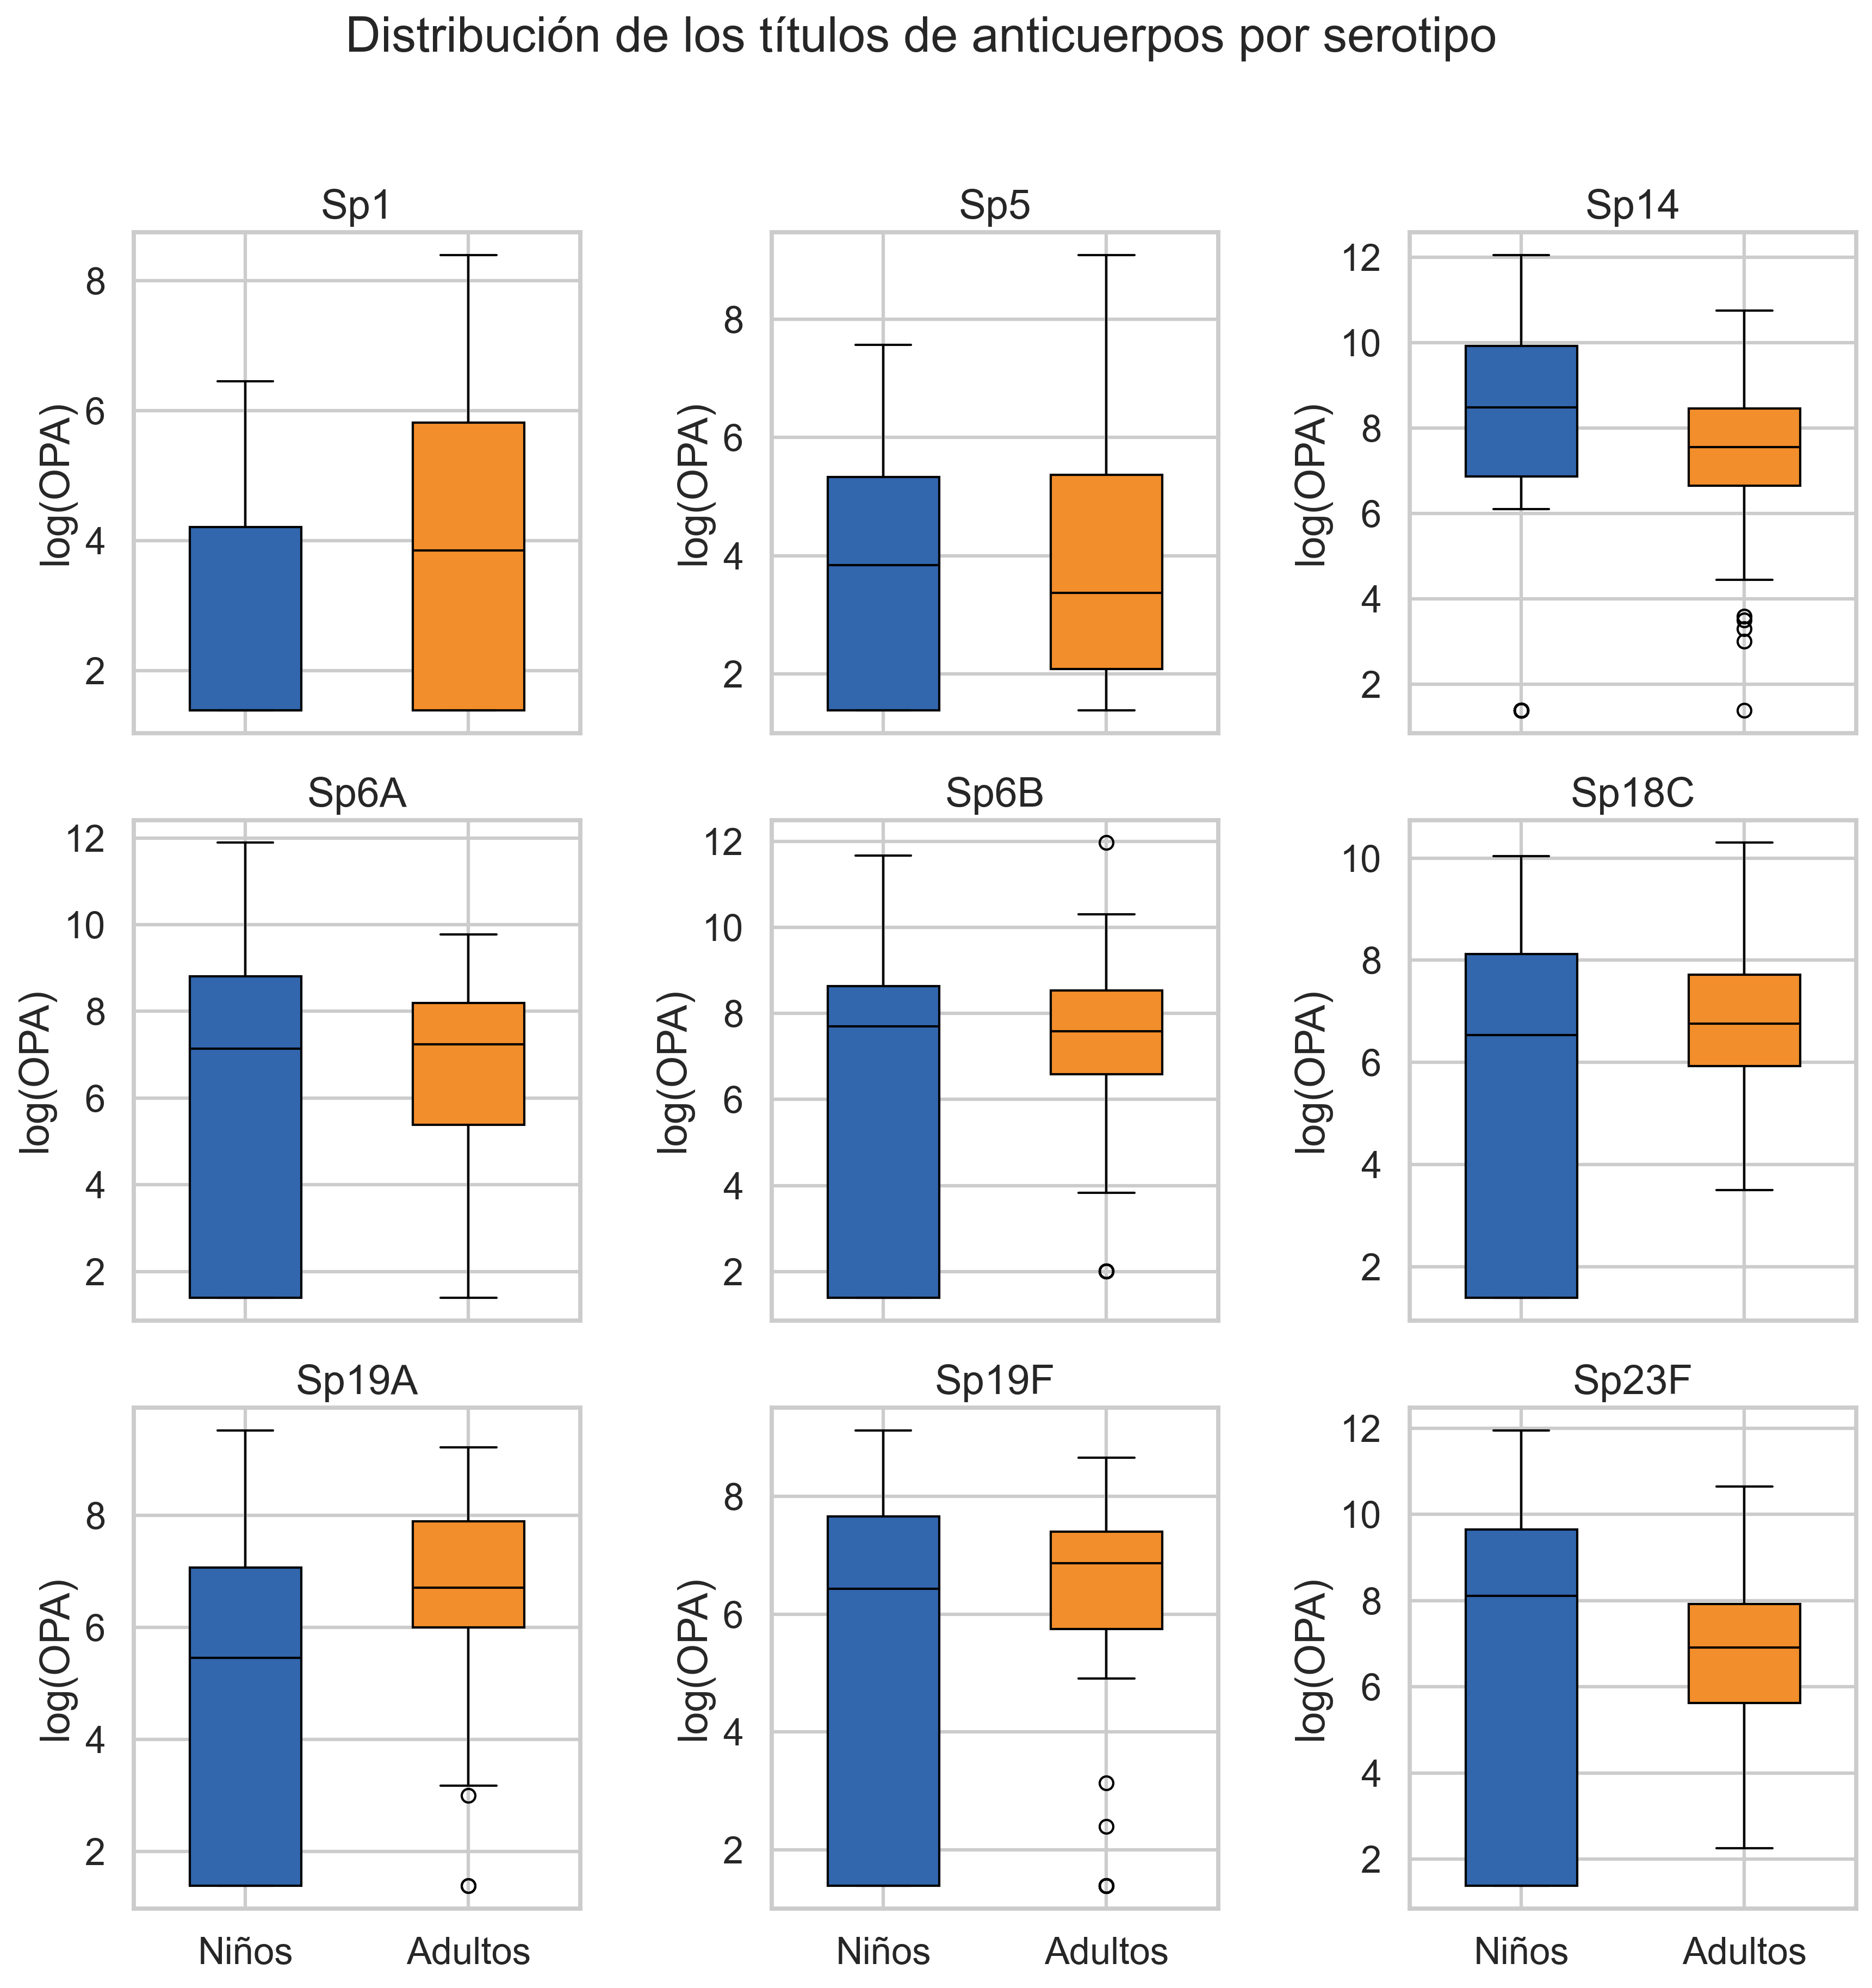
\includegraphics[width=0.8\textwidth]{Graphics/boxplot.png}
	\caption{Comparación de respuesta opsonofagocítica  (OPA) por serotipo y grupo etario.}
	\label{fig:boxplot}
\end{figure}
\FloatBarrier

\begin{figure}[ht]
	\centering
	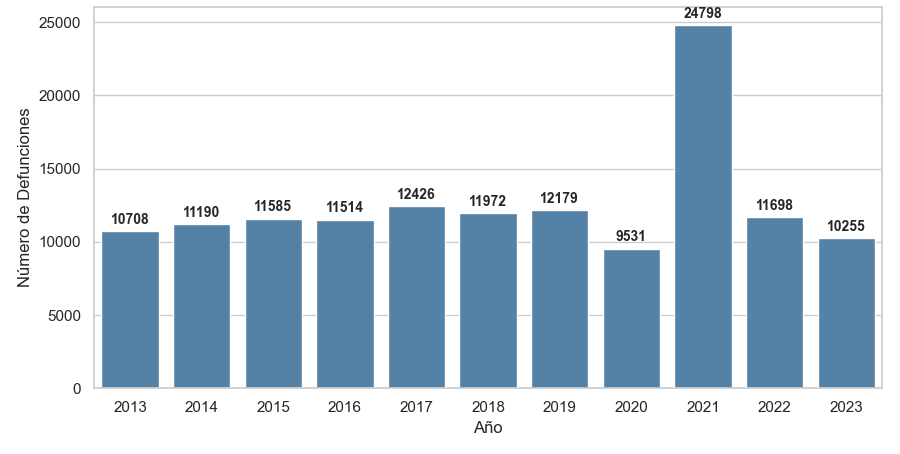
\includegraphics[width=1.0\textwidth]{Graphics/deaths_per_year.png}
	\caption{Defunciones por enfermedades neumocócicas en Cuba entre 2013 y 2023 en mayores de 60 años general.}
	\label{fig:bar_deaths}
\end{figure}
\FloatBarrier

\begin{figure}[ht]
	\centering
	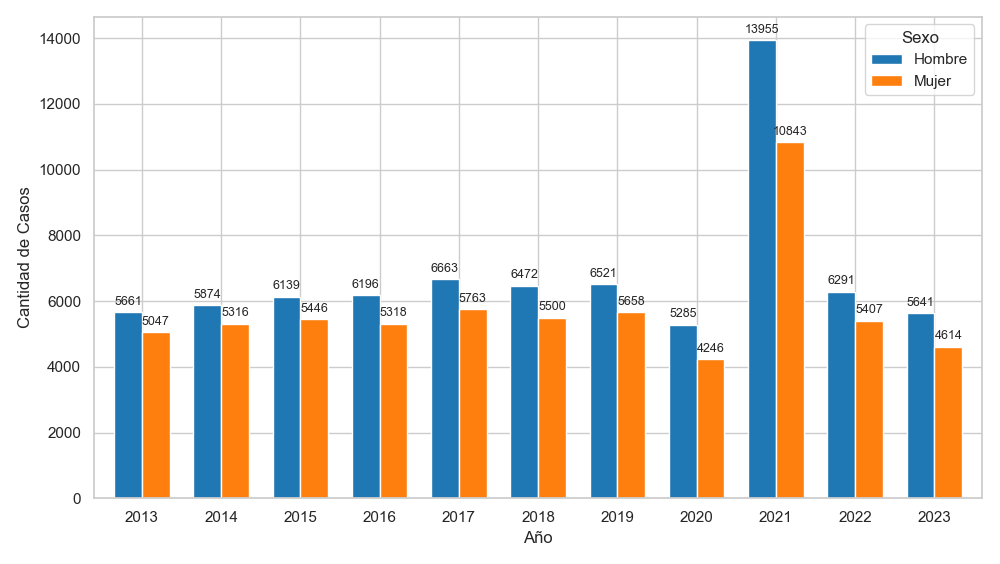
\includegraphics[width=0.8\textwidth]{Graphics/sex.png}
	\caption{Defunciones por enfermedades neumocócicas en Cuba entre 2013 y 2023 en mayores de 60 años por sexo.}
	\label{fig:bar_sex}
\end{figure}
\FloatBarrier

\begin{figure}[ht]
	\centering
	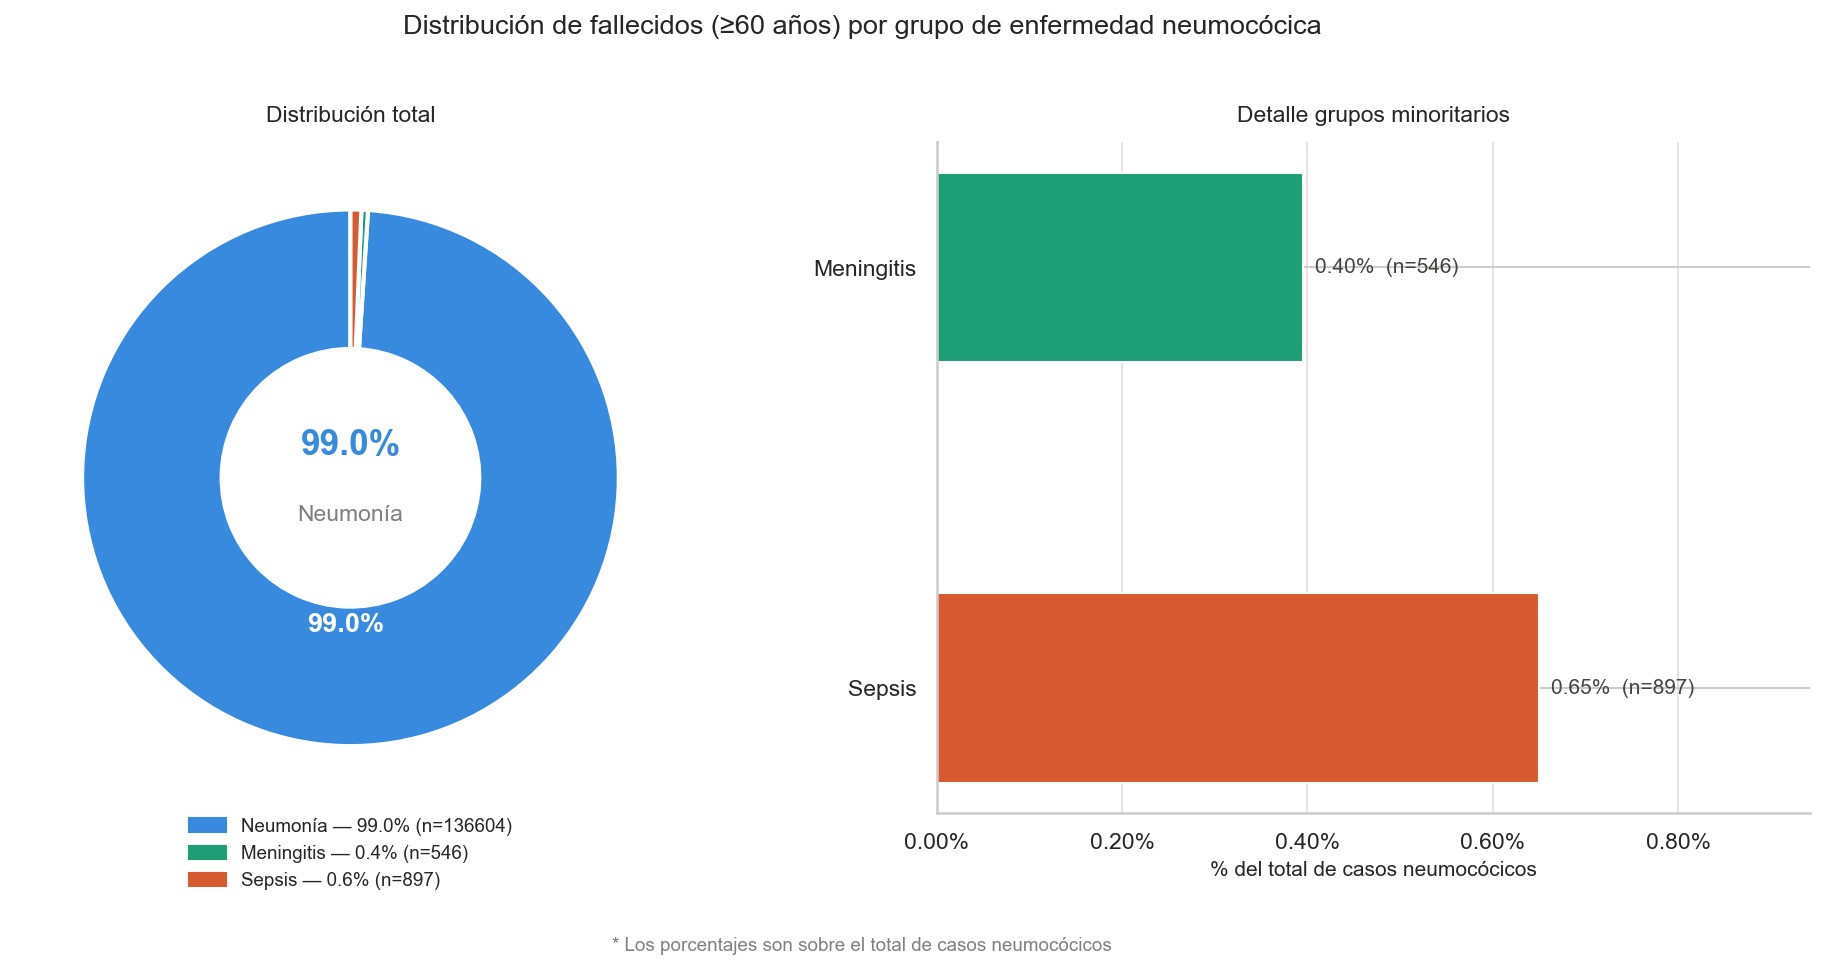
\includegraphics[width=0.9\textwidth]{Graphics/pie.png}
	\caption{Distibución de las manifestaciones clínicas de la enfermedad neumocócica en Cuba entre 2013 y 2023.}
	\label{fig:pie}
\end{figure}
\FloatBarrier

\vspace{1.5cm}
\begin{table}[htbp]
	\centering
	\caption{Intervalos de confianza usando Wald vs Perfil de Verosimilitud}
	\label{tab:wald_vs_profile}
	
	\renewcommand{\arraystretch}{1.5} 
	
	\begin{adjustbox}{max width=\textwidth}
		% Se añaden '|' entre las letras para crear las líneas verticales columna por columna
		\begin{tabular}{|l|c|c|c|c|c|c|c|c|c|}
			\hline
			& \multicolumn{3}{c|}{\textbf{Niños}} & \multicolumn{3}{c|}{\textbf{Adultos}} & \multicolumn{3}{c|}{\textbf{Razón de Medias Geométricas}} \\
			\hline
			\textbf{Serotipo} & \textbf{GMT} & \textbf{IC Wald} & \textbf{IC Verosimilitud} & \textbf{GMT} & \textbf{IC Wald} & \textbf{IC Verosimilitud} & \textbf{GMR} & \textbf{IC Wald} & \textbf{IC Verosimilitud} \\
			\hline
			Sp1   & 2.16   & [0.6, 7.8]       & [0.43, 6.34]     & 29.28   & [13.37, 64.09]   & [12.25, 61.79]   & 8.60  & [2.61, 28.36]  & [2.68, 30.68]  \\ \hline
			Sp5   & 30.15  & [16.12, 56.36]   & [15.3, 55.11]    & 38.84   & [19.89, 75.84]   & [19.12, 75.19]   & 1.28  & [0.52, 3.14]   & [0.52, 3.19]   \\ \hline
			Sp6A  & 334.20 & [129.96, 859.44] & [122.26, 844.02] & 715.48  & [421.31, 1215.05]& [416.24, 1222.73]& 1.71  & [0.6, 4.87]    & [0.6, 4.97]    \\ \hline
			Sp6B  & 418.76 & [177.19, 989.67] & [168.95, 976.91] & 1245.15 & [712.95, 2174.6]  & [706.94, 2193.1] & 2.57  & [0.94, 7.05]   & [0.94, 7.18]   \\ \hline
			Sp14  & 2194.62& [1077.42, 4470.28]& [1054.93, 4475.86]& 1504.39& [984.47, 2298.88] & [977.54, 2313.18]& 0.64  & [0.27, 1.51]   & [0.27, 1.52]   \\ \hline
			Sp18C & 74.10  & [24.31, 225.85]  & [21.61, 213.7]   & 831.14  & [576.17, 1198.93] & [572.88, 1205.83]& 6.70  & [2.43, 18.44]  & [2.46, 19.01]  \\ \hline
			Sp19A & 52.26  & [21.71, 125.83]  & [19.94, 120.97]  & 749.21  & [491.01, 1143.18] & [487.15, 1150.0] & 10.21 & [4.17, 24.99]  & [4.2, 25.63]   \\ \hline
			Sp19F & 67.36  & [24.39, 185.98]  & [22.06, 177.34]  & 498.97  & [289.23, 860.8]   & [284.31, 864.75] & 4.90  & [1.63, 14.72]  & [1.64, 15.17]  \\ \hline
			Sp23F & 472.34 & [168.72, 1322.3] & [158.14, 1293.76]& 658.27  & [404.3, 1071.77]  & [401.32, 1079.73]& 1.07  & [0.36, 3.22]   & [0.36, 3.29]   \\ 
			\hline
		\end{tabular}
	\end{adjustbox}
\end{table}
